\documentclass[letterpaper,11pt,oneside]{memoir}

\usepackage{xess}

\product[StickIt! Board]
\manualnum{002}
\manualversion{4.0}
\newcommand{\copyrightyear}{2012-2015}
\newcommand{\xula}{XuLA Board}

\begin{document}

\frontmatter

\makexessmanualtitlepage{product_cover.jpg}{0.7}

\makexesslegal{\copyrightyear}

\begin{xessrevisiontbl}
	01/15/2012 & 1.0 & Initial release for \product\ V1.0.\\
	\hline
	09/23/2012 & 2.0 & Revised for \product\ V2.0.\\
	\hline
	12/11/2012 & 3.0 & Revised for \product\ V3.0.\\
	\hline
	06/01/2015 & 4.0 & Revised for \product\ V4.0.\\
\end{xessrevisiontbl}

\makexesstoc

\mainmatter

\chapter{Preliminaries}

Here's some helpful information before getting started.


\section{Getting Help!}

Here are some places to get help if you encounter problems:

\begin{itemize}
\item If you can't get the \product\ to work, send an e-mail message
	describing your problem to \href{mailto:\helpemail}{\helpemail}. 
\item Or submit a problem report at	\url{\helppage}.
\item \href{http://www.xess.com}{Our web site} also has
	\begin{itemize}
	\item \href{http://www.xess.com/projects/}{example designs}, 
	\item \href{http://www.xess.com/appnotes/}{application notes}, and
	\item \href{http://www.xess.com/tutorials/}{tutorials}.
%	\item answers to frequently-asked-questions,
%	\item \href{}{a forum where you can post questions}.
	\end{itemize}
\end{itemize}


\section{Take Notice!}

\begin{itemize}
\item The \xula\ is not 5V-tolerant. \warning{Do not connect 5V logic signals
	to the \digpmod\ sockets of the \product.}
\item \warning{Only power the \product\ with a regulated 5 VDC,
	center-positive power supply.}
\end{itemize}


\pagebreak %%%%%%%%%%%%%%%%%%%%%%%%%%%%%%%%%%%%%%%%%%%%%%%%%%%%%%%%%%%%%%%%%%%%%%

\section{Packing List}

Here is what you should have received in your package:

\begin{itemize}
	\item a \product.
	\item a 20\by 2 socket.
	\item a 20\by 2 header.
\end{itemize}


\chapter{Setup}

The \product\ accepts a \xula\ and provides it with connections to
separate StickIt! modules such as LED displays, buttons, audio I/O, etc.

\section{Inserting a XuLA Board into Your \texorpdfstring{\product}{StickIt! Board}}

You insert a \xula\ into the central row of sockets on the \product\ as
shown below. Make sure the \xula\ prototyping header pins line-up with the sockets
and that the USB connector is oriented towards the \product\ RESET button.

\fixedpic{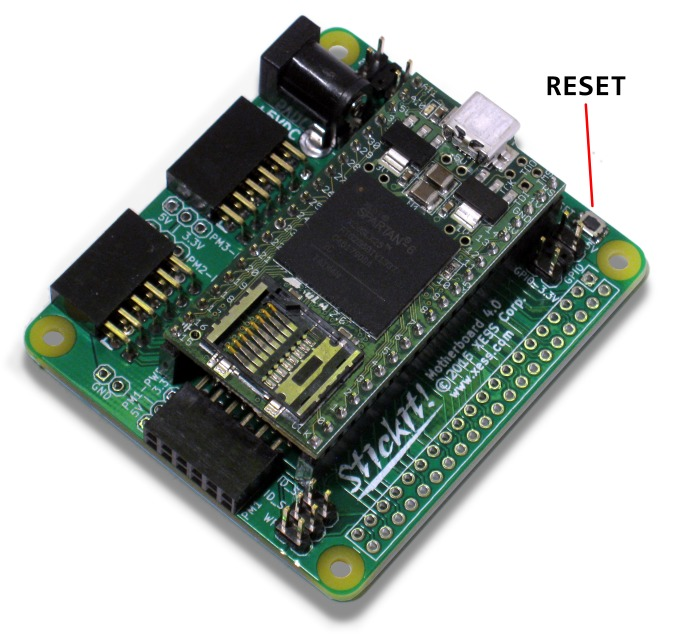
\includegraphics[width=0.7\textwidth]{stickit_with_xula.jpg}}

To insure a stable connection with the \product, the \xula\ should
have 0.025'' square posts soldered into its prototyping header. 
\warning{The 0.019'' round posts used for mounting a \xula\ into a solderless 
breadboard should not be used or else intermittent connections will occur!}

\section{Applying Power to Your \texorpdfstring{\product}{StickIt! Board}}

There are several ways to power the combination of your \xula\ and \product.
Each of these will be discussed below.

\subsection{Applying Power Through the USB Port}

Connecting the \xula\ to a USB port provides it with a 5V supply capable of
delivering up to 500 mA of current.
The 5V supply can also power the \product\ and any attached StickIt! modules by 
placing a shunt on the XULA-PWR jumper as shown below.

\fixedpic{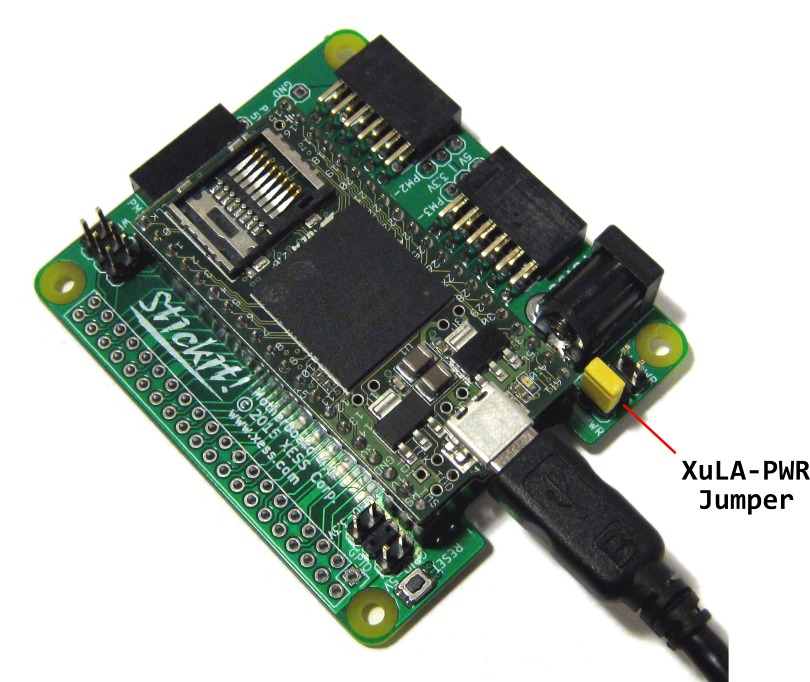
\includegraphics[width=0.7\textwidth]{XULA_PWR.jpg}}

\pagebreak %%%%%%%%%%%%%%%%%%%%%%%%%%%%%%%%%%%%%%%%%%%%%%%%%%%%%%%%%%%%%%%%%%%%%%

\subsection{Applying Power Though the Power Jack}

For applications that require more power than the USB port can provide, you can
attach a regulated, 5 VDC center-positive power adapter to the 5VDC jack on the
\product. 
In this case, the shunt should be removed from the XULA-PWR
jumper and placed on the 5V-PWR jumper as shown below. 
In this configuration, the USB port powers the \xula\ while the adapter powers
the \product\ and any attached StickIt! modules.

\fixedpic{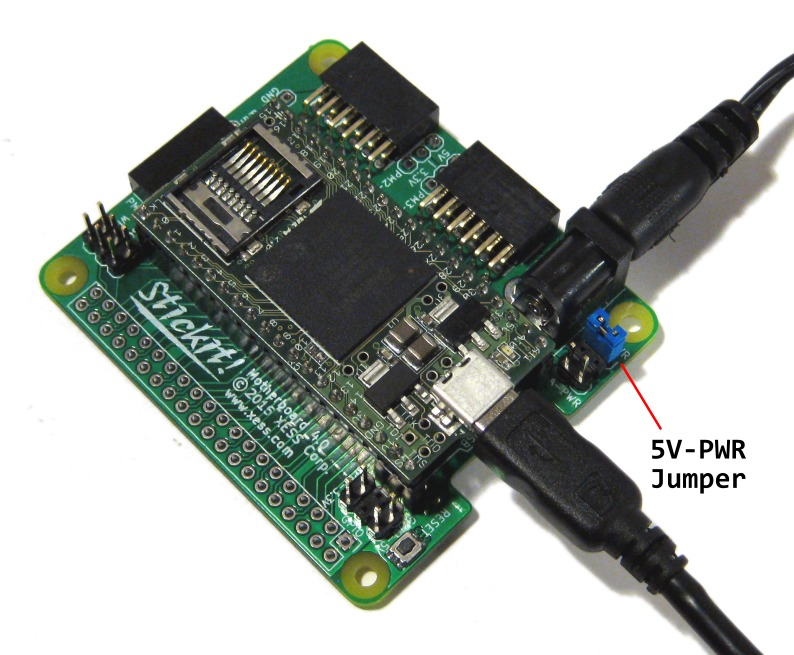
\includegraphics[width=0.7\textwidth]{5V_PWR.jpg}}

\pagebreak %%%%%%%%%%%%%%%%%%%%%%%%%%%%%%%%%%%%%%%%%%%%%%%%%%%%%%%%%%%%%%%%%%%%%%

\subsection{Applying Power to Stand-Alone Applications}

For applications that operate stand-alone with no connection to a USB port, you
can attach a regulated, 5 VDC center-positive power adapter to the 5VDC jack on
the \product. 
In addition, shunts should be placed on both the XULA-PWR
and 5V-PWR jumpers as shown below. 
This will transfer power from the adapter through the \product\ to the \xula.

\fixedpic{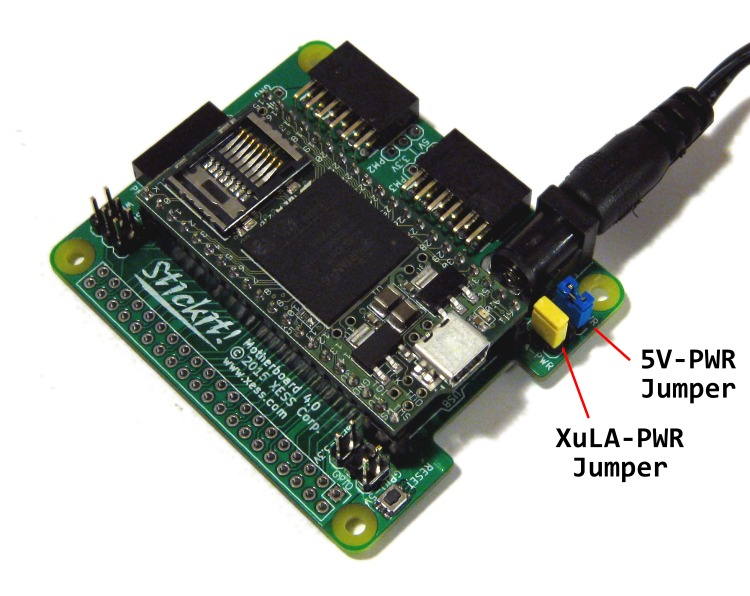
\includegraphics[width=0.7\textwidth]{Standalone_PWR.jpg}}

\warning{A USB cable should not be attached to the \xula\ in this
configuration or damage may result from the direct connection of the power
adapter to the 5V supply pin of the USB port!}

In order to prevent inadvertent damage, you can remove the shunt on 5V jumper of the
\xula\ to disconnect the USB 5V supply as shown below. Note that doing this will
prevent you from powering the \xula\ through the USB port until the 5V shunt is
restored.
\warning{By default, the 5V jumper is closed by a wire trace on the underside
of the \xula! You will need to cut this trace to open the jumper.} 

\pagebreak %%%%%%%%%%%%%%%%%%%%%%%%%%%%%%%%%%%%%%%%%%%%%%%%%%%%%%%%%%%%%%%%%%%%%%

\subsection{Applying Power from a \rpi}

The \product\ can get power through the GPIO connector of a \rpi\
by placing a shunt on the GPIO-5V jumper.
This connects the 5V supply from the \rpi\ to the same power rail as the 5V power jack.
Because of this, \warning{a power adapter should not be connected to the 5V jack in this
configuration or damage may result from the direct connection of the power
adapter to the 5V supply of the \rpi!}
A power adapter \emphasis{can} be used to power the \product\ when it is attached
to a \rpi\ only if the shunt is removed from the GPIO-5V jumper.
In addition, \warning{a shunt should \emphasis{never} be placed on the GPIO-3.3V jumper 
when the \product\ is attached to the \rpi.}

\fixedpic{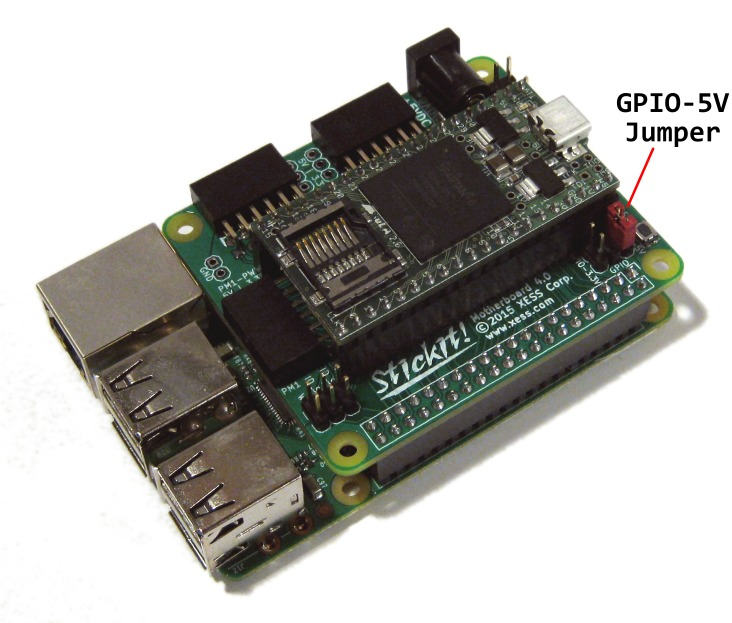
\includegraphics[width=0.7\textwidth]{RPI_PWR.jpg}}


\chapter{Connections}

This chapter describes the various sections of the \product\ and shows how
the \xula\ I/O connects to them.
In addition to the partial schematics that follow, you can find a 
complete schematic at the end of this manual.


\section{XuLA Board Socket}

A \xula\ connects to the \product\ through the J1 socket.

\fixedpic{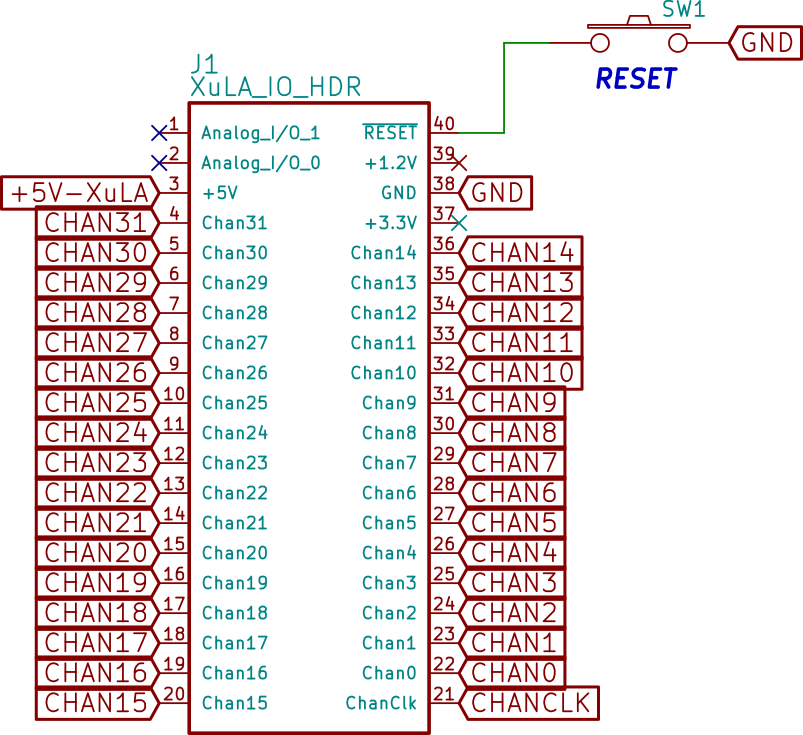
\includegraphics[width=0.5\textwidth]{XuLA_socket.png}}

Please note the following:

\begin{itemize}
\item The \xula\ 5V pin is connected to the +5V-XULA signal on the \product.
	This allows the \xula\ to send power to or receive power from the \product.
	This is the only voltage supply shared by both the \xula\ and the \product.
\item The \xula\ 3.3V and 1.2V pins do not connect to anything else on the \product.
\item The \xula\ ground is connected to the \product\ ground.
\item The reset pin of the \xula\ connects to the to the RESET button 
	on the \product. Pushing this button resets the \xula.
\item The analog I/O pins of the \xula\ do not connect to anything else 
	on the \product.
\end{itemize}

Here are the FPGA pins connected to each channel for both the XuLA and XuLA2 Boards:

\begin{center}
\renewcommand{\arraystretch}{1.3}
\begin{tabu}{|l|l|l|c||c|l|l|l|}
\hline
\xesstblhdr
XuLA & XuLA2 & J1 & \multicolumn{2}{c|}{Pin\#} & J1 & XuLA2 & XuLA\\
\hline\hline
AN1 & AN1  &      & 1  & 21 & RESET & RESET & RESET \\\hline
AN0 & AN0  &      & 2  & 22 &       & +1.2V & +1.2V \\\hline
+5V & +5V  & +5V  & 3  & 23 & GND   & GND   & GND   \\\hline
P88 & A2   & CH31 & 4  & 24 &       & +3.3V & +3.3V \\\hline
P89 & B2   & CH30 & 5  & 25 & CH14  & B15   & P84   \\\hline
P93 & B1   & CH29 & 6  & 26 & CH13  & B16   & P83   \\\hline
P94 & C1   & CH28 & 7  & 27 & CH12  & C15   & P82   \\\hline
P97 & E2   & CH27 & 8  & 28 & CH11  & C16   & P73   \\\hline
P3  & E1   & CH26 & 9  & 29 & CH10  & F16   & P72   \\\hline
P4  & F2   & CH25 & 10 & 30 & CH9   & F15   & P68   \\\hline
P7  & F1   & CH24 & 11 & 31 & CH8   & J14   & P62   \\\hline
P12 & H2   & CH23 & 12 & 32 & CH7   & J16   & P61   \\\hline
P13 & H1   & CH22 & 13 & 33 & CH6   & K16   & P57   \\\hline
P19 & J4   & CH21 & 14 & 34 & CH5   & K15   & P56   \\\hline
P20 & K3   & CH20 & 15 & 35 & CH4   & M16   & P52   \\\hline
P21 & M1   & CH19 & 16 & 36 & CH3   & M15   & P50   \\\hline
P32 & M2   & CH18 & 17 & 37 & CH2   & R16   & P39   \\\hline
P33 & R1   & CH17 & 18 & 38 & CH1   & R15   & P37   \\\hline
P34 & R2   & CH16 & 19 & 39 & CH0   & R7    & P36   \\\hline
P35 & T4   & CH15 & 20 & 40 & CHCLK & T7    & P44   \\\hline
\end{tabu}
\label{tab:ChanneltoFPGAConnections}
\end{center}


\pagebreak %%%%%%%%%%%%%%%%%%%%%%%%%%%%%%%%%%%%%%%%%%%%%%%%%%%%%%%%%%%%%%%%%%%%%%

\section{Power Circuitry}

The \product\ accepts +5V from either
\begin{itemize} 
\item a \xula\ (when there is a shunt on the XULA-PWR jumper),
\item an external power adapter (when there is a shunt on the 5V-PWR jumper), or
\item a \rpi (when there is a shunt on the GPIO-5V jumper).
\end{itemize}

The \product\ voltage regulator creates the +3.3V supply.

\fixedpic{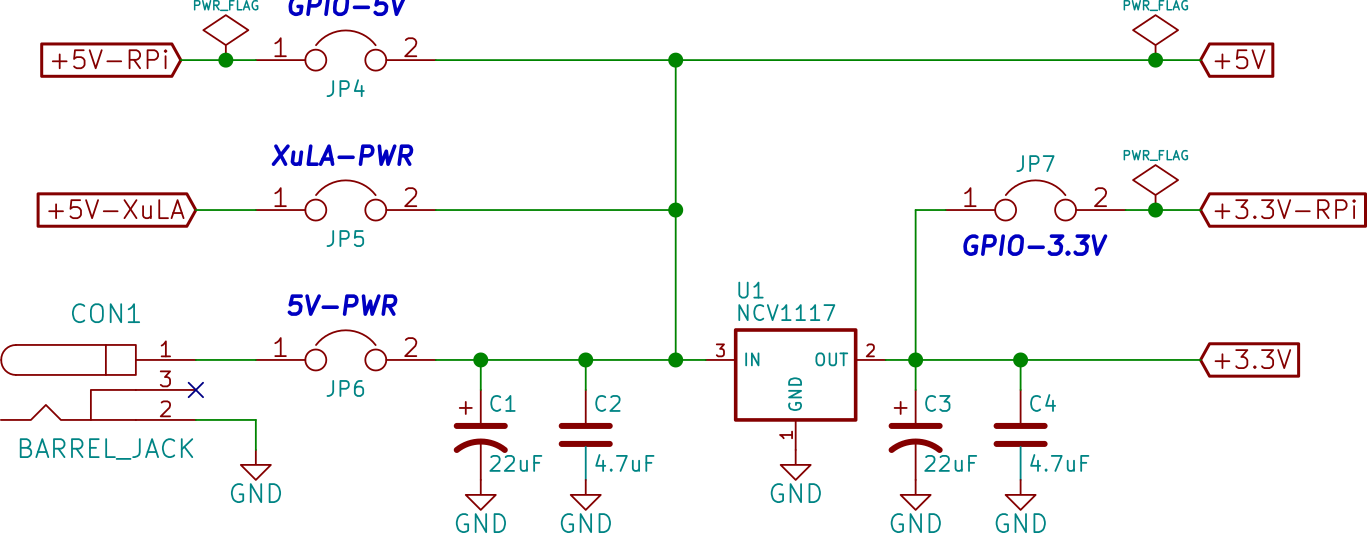
\includegraphics[width=0.7\textwidth]{pwr_circuit.png}}

Be aware that placing shunts on both the XULA-PWR and 5V-PWR jumpers will
connect the external power adapter to the \xula\ power supply. 
\warning{This will cause damage} unless 1) the USB cable is removed from the \xula,
or 2) the 5V jumper on the \xula\ is open.
(Note that in its factory-original
configuration, the 5V jumper on the \xula\ is shorted by a wiring trace on
the bottom of the PCB which must be cut to disconnect the 5V supply from the
USB port.)

Also be aware that placing shunts on both the XuLA-PWR and GPIO-5V jumpers
when the \product\ is attached to a \rpi\
will connect the external power adapter to the \rpi\ 5V supply.
\warning{This will cause damage!}
There must \emphasis{never} be a shunt on both the XuLA-PWR and GPIO-5V jumpers 
when the \product\ is attached to a \rpi.


\pagebreak %%%%%%%%%%%%%%%%%%%%%%%%%%%%%%%%%%%%%%%%%%%%%%%%%%%%%%%%%%%%%%%%%%%%%%

\section{\digpmod\ Sockets}

There are three sockets (PM1\textendash PM3) for connecting external \digpmod\ modules 
to the \product.
All of these sockets accept either four-bit or eight-bit \digpmod\ modules.
(There are also five sockets for connecting 
\href{http://www.seeedstudio.com/wiki/Category:Grove}{Grove boards},
but these are covered by the \digpmod\ sockets and can't be used. 
Just ignore them. 
Really, act like they're not even there.)

\fixedpic{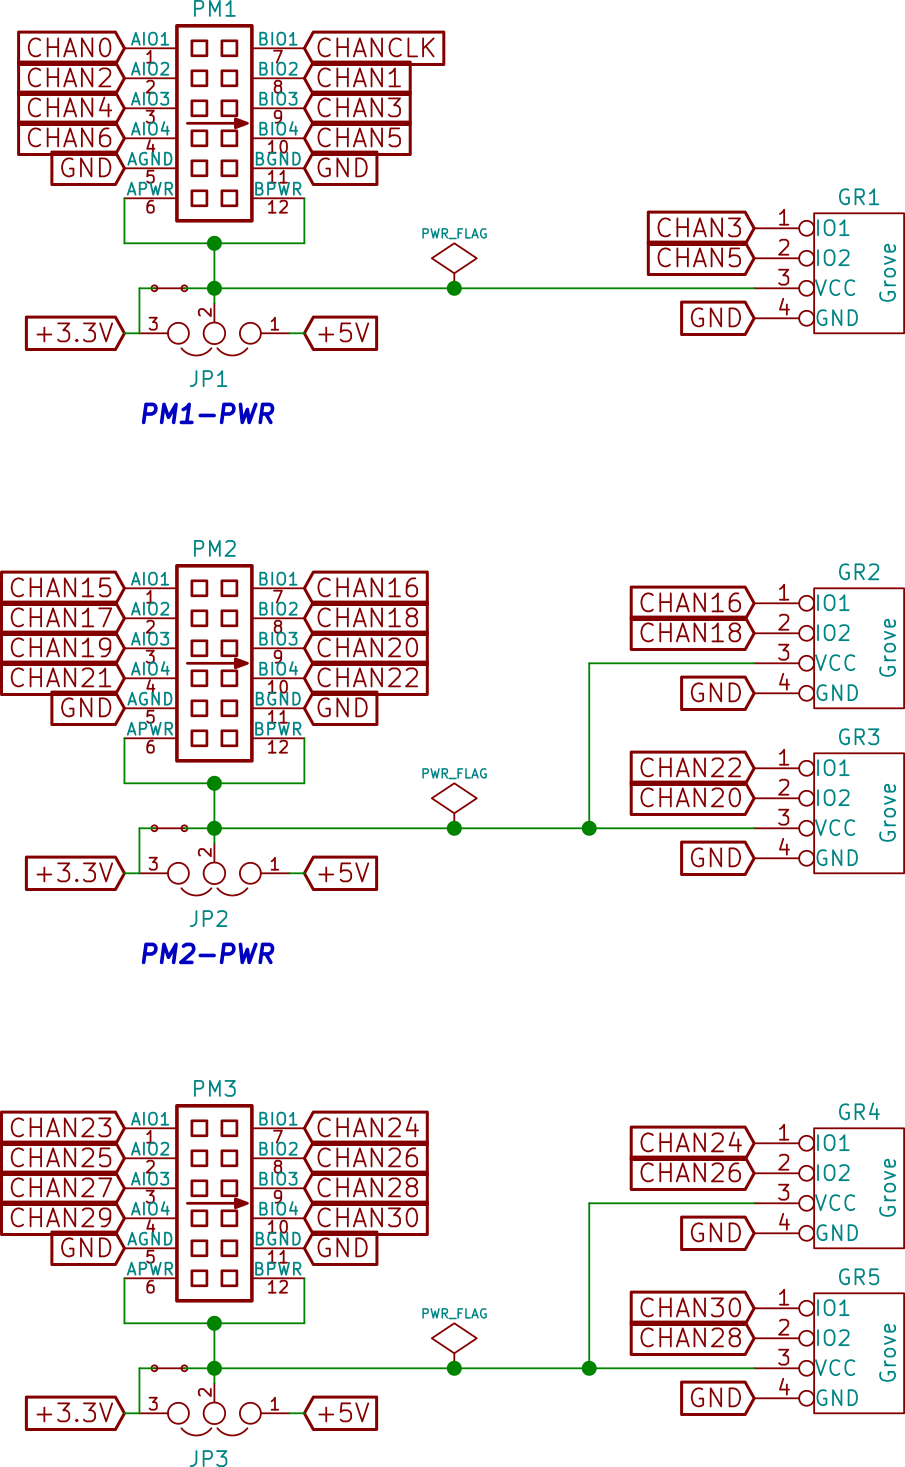
\includegraphics[width=0.5\textwidth]{pmod_sockets.png}}

\pagebreak %%%%%%%%%%%%%%%%%%%%%%%%%%%%%%%%%%%%%%%%%%%%%%%%%%%%%%%%%%%%%%%%%%%%%%

A total of 24 channels connect from the \xula\ to the \digpmod\
sockets, so you can use any combination of modules that require 24 total I/Os or less.
The channel connections to each of the \digpmod\ sockets are shown in the 
following table:

\begin{center}
\renewcommand{\arraystretch}{1.3}
\begin{tabu}{|l|l|c||c|l|l|}
\hline
\xesstblhdr
Chan & \digpmod\ I/O & \multicolumn{2}{c|}{Pin\#} & \digpmod\ I/O & Chan\\
\hline\hline
\multicolumn{6}{|c|}{\cellcolor[gray]{0.7} PM1}\\
\hline
CH0  & D0     &  1 &  7 & D1     & CHCLK \\\hline
CH2  & D2     &  2 &  8 & D3     & CH1   \\\hline
CH4  & D4     &  3 &  9 & D5     & CH3   \\\hline
CH6  & D6     &  4 & 10 & D7     & CH5   \\\hline
     & GND    &  5 & 11 & GND    &       \\\hline
     & VCC    &  6 & 12 & VCC    &       \\\hline
\hline
\multicolumn{6}{|c|}{\cellcolor[gray]{0.7} PM2}\\
\hline
CH15 & D0     &  1 &  7 & D1     & CH16  \\\hline
CH17 & D2     &  2 &  8 & D3     & CH18  \\\hline
CH19 & D4     &  3 &  9 & D5     & CH20  \\\hline
CH21 & D6     &  4 & 10 & D7     & CH22  \\\hline
     & GND    &  5 & 11 & GND    &       \\\hline
     & VCC    &  6 & 12 & VCC    &       \\\hline
\hline
\multicolumn{6}{|c|}{\cellcolor[gray]{0.7} PM3}\\
\hline
CH23 & D0     &  1 &  7 & D1     & CH24  \\\hline
CH25 & D2     &  2 &  8 & D3     & CH26  \\\hline
CH27 & D4     &  3 &  9 & D5     & CH28  \\\hline
CH29 & D6     &  4 & 10 & D7     & CH30  \\\hline
     & GND    &  5 & 11 & GND    &       \\\hline
     & VCC    &  6 & 12 & VCC    &       \\\hline
\end{tabu}
\label{tab:ChanneltoPMODConnections}
\end{center}

\pagebreak %%%%%%%%%%%%%%%%%%%%%%%%%%%%%%%%%%%%%%%%%%%%%%%%%%%%%%%%%%%%%%%%%%%%%%

The physical arrangement of the \digpmod\ I/O signals is shown below.

\fixedpic{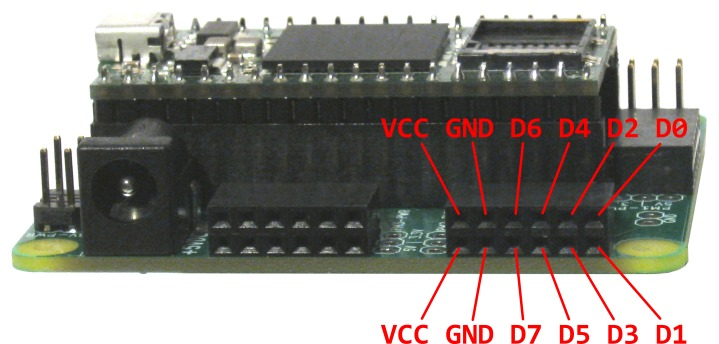
\includegraphics[width=0.7\textwidth]{PMOD_socket.jpg}}

Each \digpmod\ socket has an associated jumper to connect either the 3.3V or 5V power
supply to the attached module. 
In their factory-original configuration, each of these jumpers is set to 3.3V 
by a shorting trace on the bottom of the \product\ PCB. 
You must cut this trace and install a jumper and shunt if you want to use a 5V module.

\fixedpic{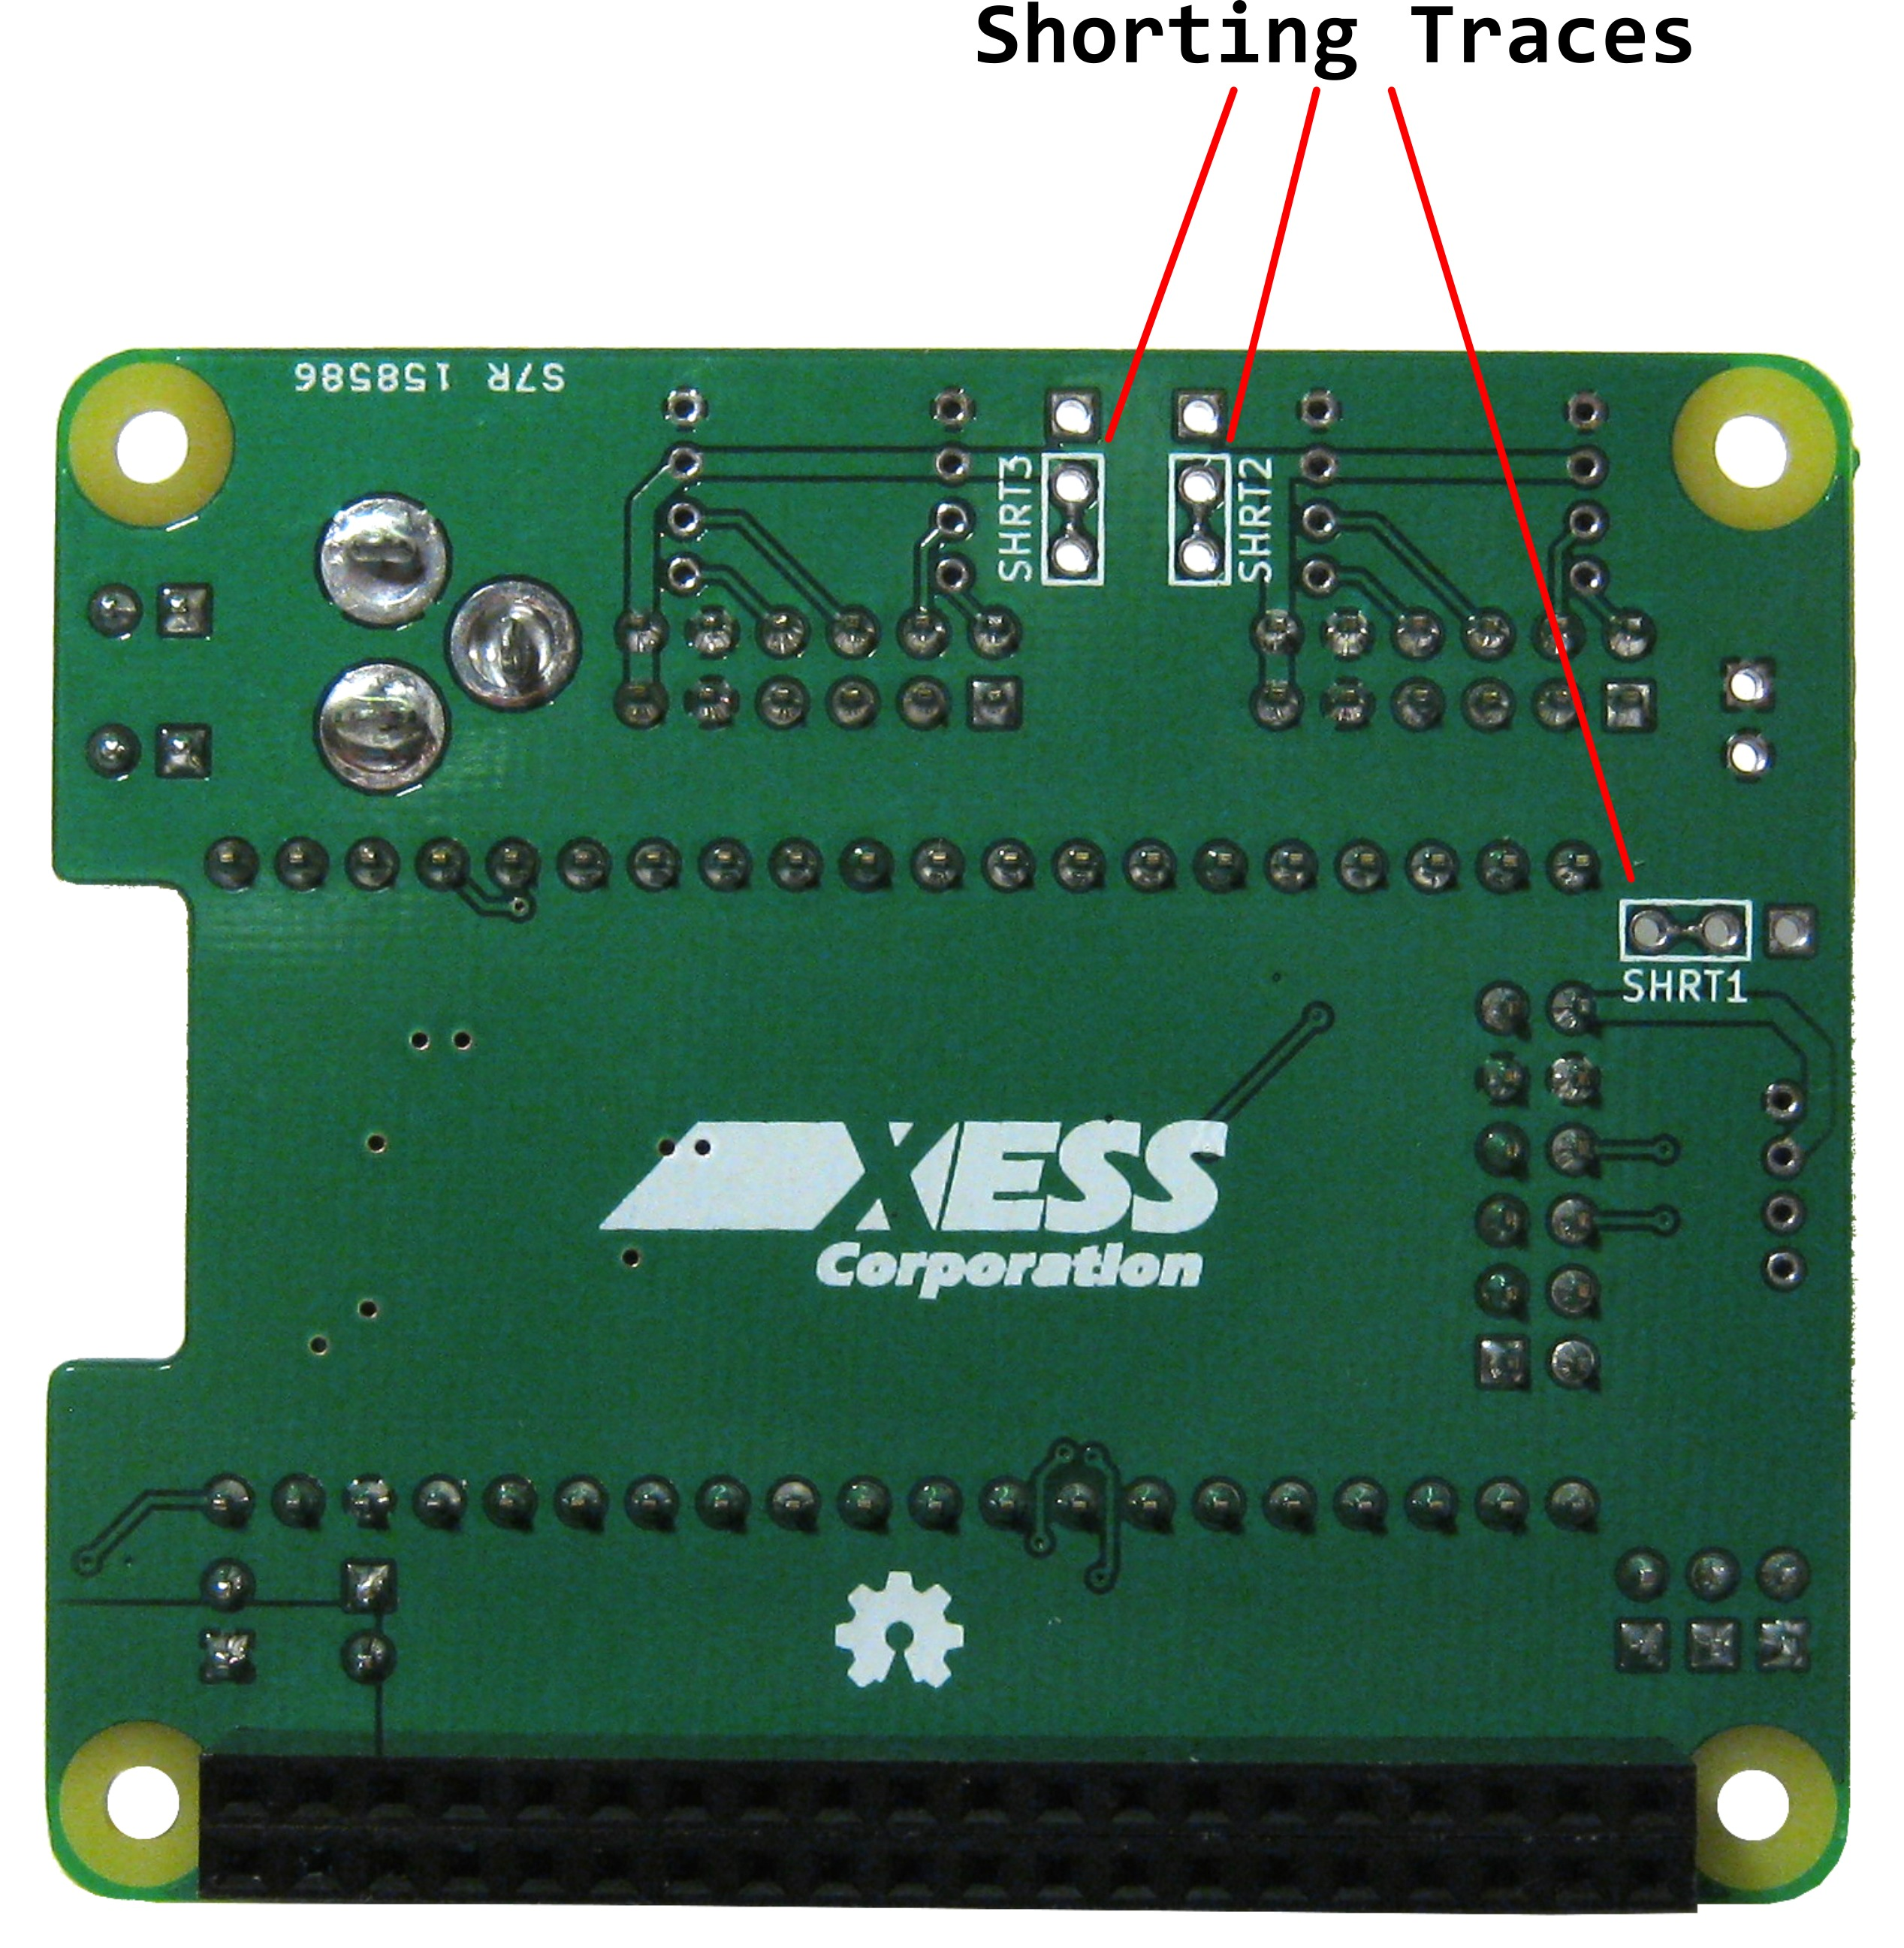
\includegraphics[width=0.7\textwidth]{shorting_traces.jpg}}


\section{\rpi\ GPIO Connector}

You can solder a 20\by 2 socket to the GPIO port of the \product\ 
so it can be connected to a \rpi.
The GPIO port provides 26 general-purpose I/O pins (the rest are for power, ground,
and access to the serial EEPROM on the \product.)

\fixedpic{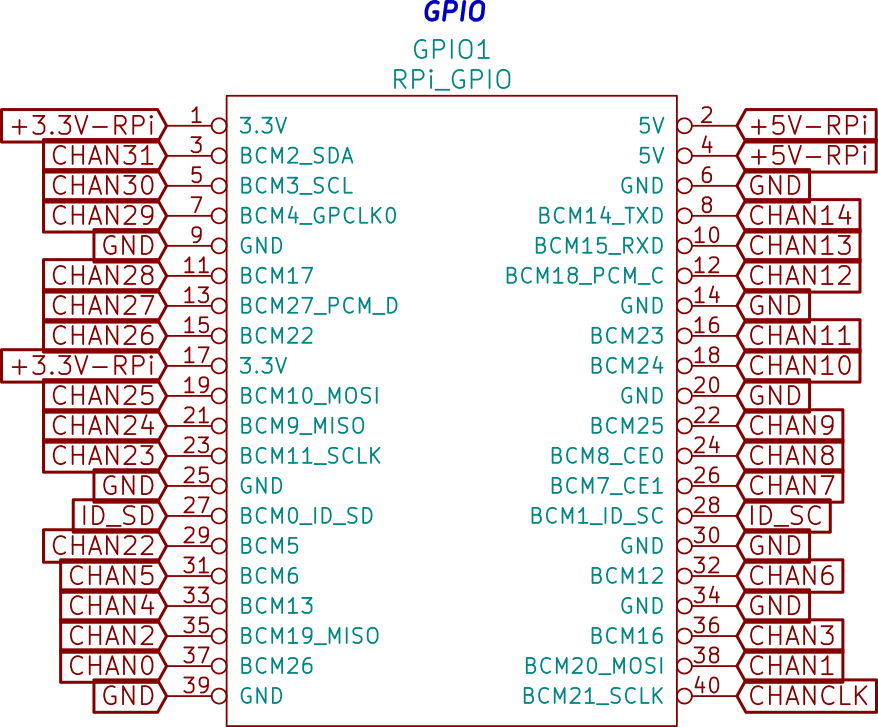
\includegraphics[width=0.5\textwidth]{rpi_socket.png}}

\pagebreak %%%%%%%%%%%%%%%%%%%%%%%%%%%%%%%%%%%%%%%%%%%%%%%%%%%%%%%%%%%%%%%%%%%%%%

The channel connections to the GPIO are shown in the following table:

\begin{center}
\renewcommand{\arraystretch}{1.3}
\begin{tabu}{|l|l|c||c|l|l|}
\hline
\xesstblhdr
Chan & RPi I/O & \multicolumn{2}{c|}{Pin\#} & RPi I/O & Chan\\\hline
\hline
     & +3.3V         &  1 &  2 & +5V           &       \\\hline
CH31 & BCM2\_SDA     &  3 &  4 & +5V           &       \\\hline
CH30 & BCM2\_SCL     &  5 &  6 & GND           &       \\\hline
CH29 & BCM4\_GPCLK0  &  7 &  8 & BCM14\_TXD    & CH14  \\\hline
     & GND           &  9 & 10 & BCM15\_RXD    & CH13  \\\hline
CH28 & BCM17         & 11 & 12 & BCM18\_PCM\_C & CH12  \\\hline
CH27 & BCM27\_PCM\_D & 13 & 14 & GND           &       \\\hline
CH26 & BCM22         & 15 & 16 & BCM23         & CH11  \\\hline
     & +3.3V         & 17 & 18 & BCM24         & CH10  \\\hline
CH25 & BCM10\_MOSI   & 19 & 20 & GND           &       \\\hline
CH24 & BCM9\_MISO    & 21 & 22 & BCM25         & CH9   \\\hline
CH23 & BCM11\_SCLK   & 23 & 24 & BCM8\_CE0     & CH8   \\\hline
     & GND           & 25 & 26 & BCM7\_CE1     & CH7   \\\hline
     & BCM0\_ID\_SD  & 27 & 28 & BCM1\_ID\_SC  &       \\\hline
CH22 & BCM5          & 29 & 30 & GND           &       \\\hline
CH5  & BCM6          & 31 & 32 & BCM12         & CH6   \\\hline
CH4  & BCM13         & 33 & 34 & GND           &       \\\hline
CH2  & BCM19\_MISO   & 35 & 36 & BCM16         & CH3   \\\hline
CH0  & BCM26         & 37 & 38 & BCM20\_MOSI   & CH1   \\\hline
     & GND           & 39 & 40 & BCM21\_SCLK   & CHCLK \\\hline
\end{tabu}
\label{tab:ChanneltoGPIOConnections}
\end{center}

You can also use the GPIO port to connect the \product\ to other pieces of
external circuitry.
When doing this, you can place shunts on the GPIO-5V and GPIO-3.3V jumpers to 
provide power to the external circuitry if needed.
However, \warning{never place a shunt on the GPIO-3.3V jumper if the external
circuitry is generating its own 3.3V supply voltage!}
The \product\ is able to supply 3.3V to other circuitry, but it cannot accept it.


\pagebreak %%%%%%%%%%%%%%%%%%%%%%%%%%%%%%%%%%%%%%%%%%%%%%%%%%%%%%%%%%%%%%%%%%%%%%

\section{HAT EEPROM}

In accordance with the 
\href{https://github.com/raspberrypi/hats}{\rpi\ HAT (Hardware Attached on Top) requirements},
the \product\ has an EEPROM that stores information about the device and how it
connects to the \rpi.

\fixedpic{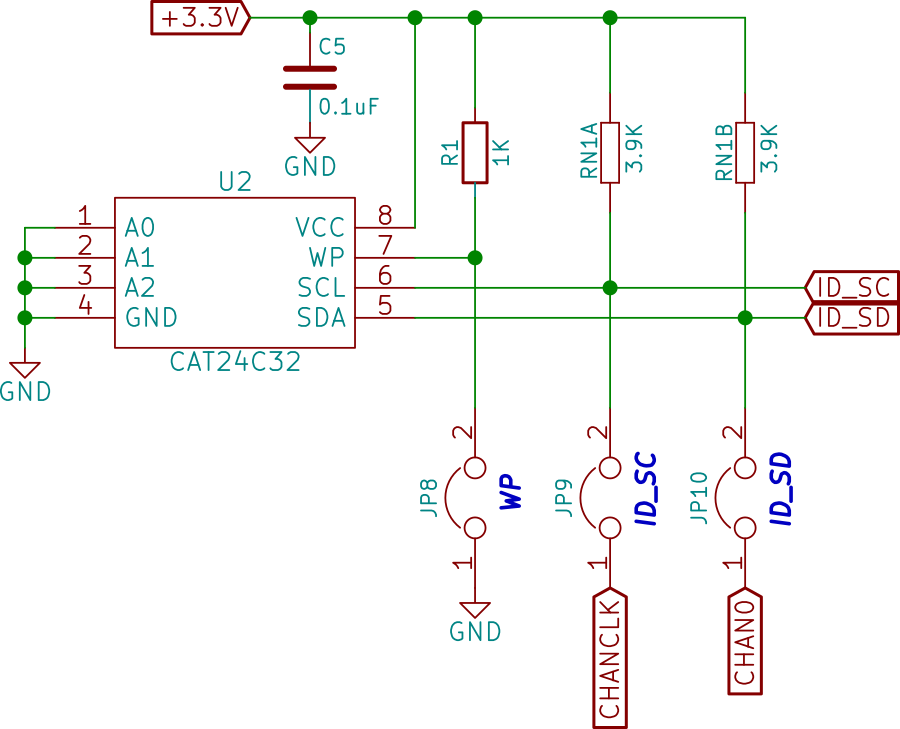
\includegraphics[width=0.5\textwidth]{eeprom.png}}

During normal operation, the EEPROM contents are read by the \rpi\ so that it can see
what GPIO pins are used by the \xula\ inserted in the \product.
In order to program the EEPROM with that information, you must place a shunt on
the WP jumper to disable the write-protect function.
The \rpi\ can then load the EEPROM through the ID\_SC and ID\_SD pins of the 
GPIO header.
(Read more about this process on page~\pageref{sec:GPIOConfig}.)

The EEPROM can also be loaded by the \xula\ (if programmed appropriately) by placing shunts
on the ID\_SC and ID\_SD jumpers as well as the WP jumper.


\chapter{Using Modules}

The \product\ serves as a means of connecting a \xula\ to various pieces of
electronics, be they \digpmod s, a \rpi, or just some generic circuitry.
The details of how this is done are presented below.

\section{Using \digpmod s}

To use the functions of a particular \digpmod, you have to determine which
I/O signals of the module are connected to which pins of the FPGA.
This is complicated by the fact the module could be plugged into any of the
\digpmod\ sockets.
As with many things in life, there's a hard way to figure this out, and an easy way.

\subsection{The Hard Way}

You can manually trace the connection of a \digpmod's I/O signals to the
FPGA pins using the following procedure:

\begin{itemize}
\item Select a \digpmod\ socket to attach the module to.
\item Use the \hyperref[tab:ChanneltoPMODConnections]{table} on page~\pageref{tab:ChanneltoPMODConnections} to determine 
	which module I/O signal terminates on each channel of the \digpmod\ socket.
\item Find which FPGA pin of the \xula\ connects to each channel using the
	\hyperref[tab:ChanneltoFPGAConnections]{table} on page~\pageref{tab:ChanneltoFPGAConnections}.
\item Make a UCF file associating each FPGA pin with each I/O of the module.
\item Include the UCF file in your Xilinx ISE FPGA project.
\end{itemize}

\pagebreak %%%%%%%%%%%%%%%%%%%%%%%%%%%%%%%%%%%%%%%%%%%%%%%%%%%%%%%%%%%%%%%%%%%%%%

As an example, consider a simple \digpmod\ with four LEDs, each
connected to one of the I/O signals like so:

\fixedpic{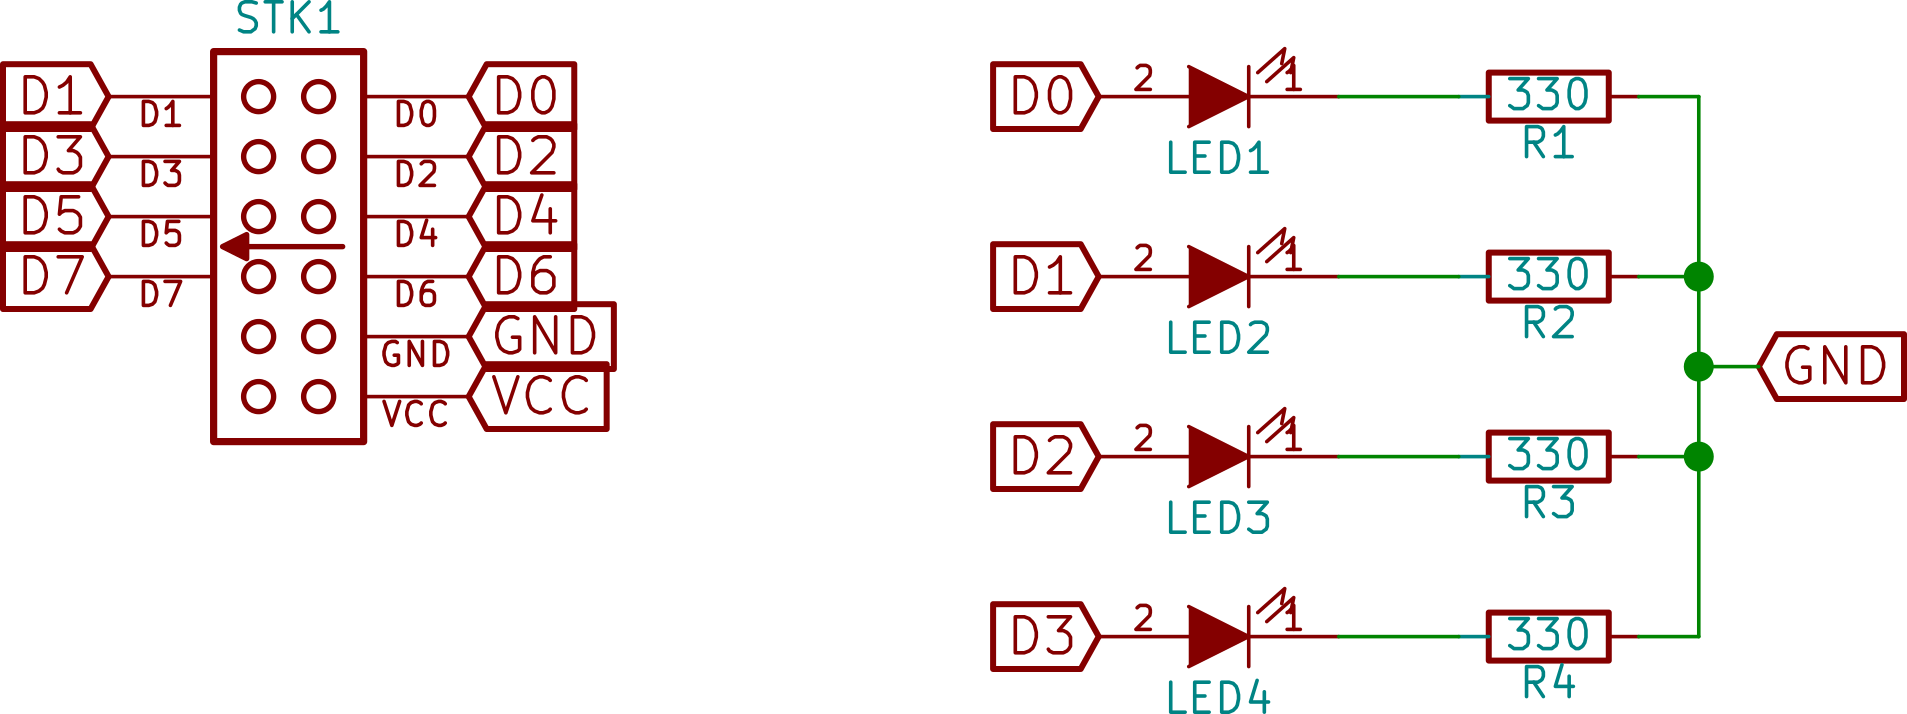
\includegraphics[width=0.5\textwidth]{pmod_example_schematic.png}}

The PCB wiring associated with this module looks like so:

\fixedpic{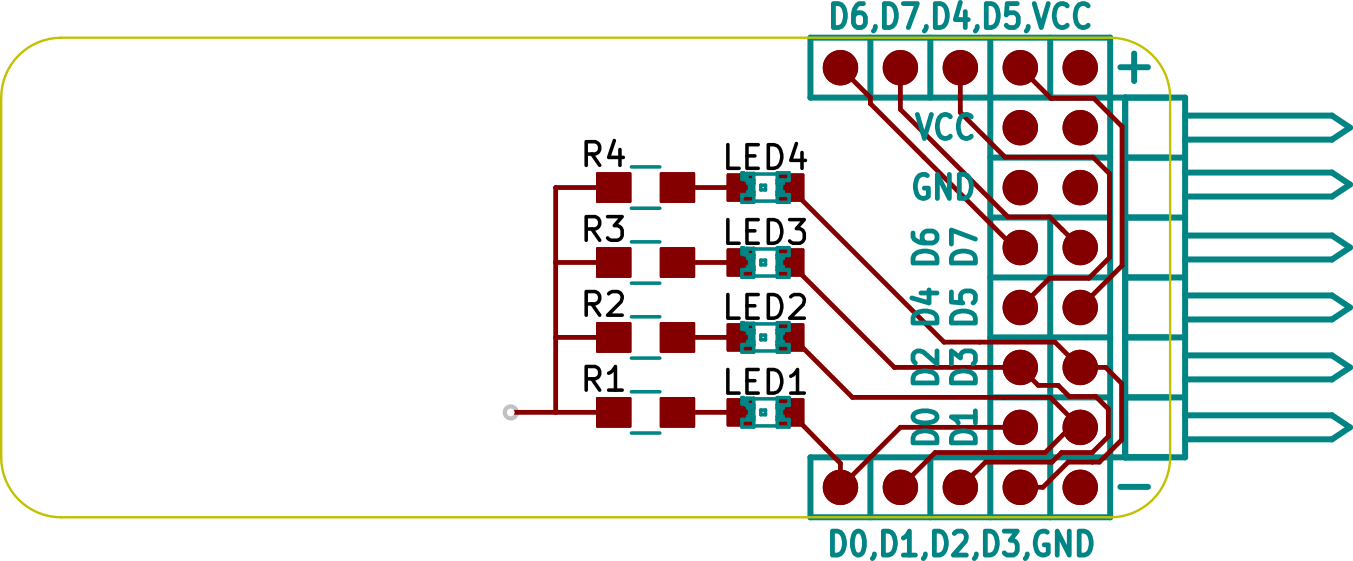
\includegraphics[width=0.5\textwidth]{pmod_example_pcb.png}}

From this, you can determine the following connections of the LEDs to the pins
of the \digpmod\ socket:

\begin{lstlisting}
LED1   D0
LED2   D1
LED3   D2
LED4   D3
\end{lstlisting}

If this module is attached to \digpmod\ socket PM3 on the \product, 
then the channel connections are:

\begin{lstlisting}
LED1   CH23  # PM3 D0
LED2   CH24  # PM3 D1
LED3   CH25  # PM3 D2
LED4   CH26  # PM3 D3
\end{lstlisting}

Now, assuming a XuLA2 Board is plugged into the \product, the mapping of
the channels to the FPGA pins is:

\begin{lstlisting}
CH23   H2  # PM3 D0
CH24   F1  # PM3 D1
CH25   F2  # PM3 D2
CH26   E1  # PM3 D3
\end{lstlisting}

From this, you can store the following pin assignments in a UCF file:

\begin{lstlisting}
NET LED1 LOC = H2;  # LED1 -> PM3-D0 -> CH23 -> H2
NET LED2 LOC = F1;  # LED2 -> PM3-D1 -> CH24 -> F1
NET LED3 LOC = F2;  # LED3 -> PM3-D2 -> CH25 -> F2
NET LED4 LOC = E1;  # LED4 -> PM3-D3 -> CH26 -> E1
\end{lstlisting}

Then include this UCF file in your ISE project.


\subsection{The Easy Way}

Tracing the paths a module's I/O signals take through a particular \digpmod\
socket to a channel which then connects to an FPGA pin is a tedious, error-prone process.
The \pgm{xsconnect}\ Python package (\url{https://pypi.python.org/pypi/xsconnect})
provides two scripts to make the process easier.

\pgm{xsconn} is the command-line script for generating pin assignments:

\begin{lstlisting}
usage: xsconn.py [-h] [-v] [-p [PERIPHERALBOARD]] [-m [MOTHERBOARD]]
                 [-d [DAUGHTERBOARD]] [-n [PORTNAME]] [-l]

optional arguments:
  -h, --help            show this help message and exit
  -v, --version         show program's version number and exit
  -p [PERIPHERALBOARD], --peripheralboard [PERIPHERALBOARD]
  -m [MOTHERBOARD], --motherboard [MOTHERBOARD]
  -d [DAUGHTERBOARD], --daughterboard [DAUGHTERBOARD]
  -n [PORTNAME], --portname [PORTNAME]
  -l, --list
\end{lstlisting}
      
For example, if a StickIt! LEDDigits peripheral board is connected to
the PM3 port of the \product\ which in turn holds a XuLA2 FPGA board, 
then the command:

\begin{lstlisting}
xsconn -p leddigits -m stickit4 -n pm3 -d xula2
\end{lstlisting}
    
will generate the output:

\begin{lstlisting}
########################################################################
# StickIt! LED Digits V2 ==[pm3]==> StickIt! V4 ==> XuLA2
net s0 loc = h2;
net s1 loc = f1;
net s2 loc = f2;
net s3 loc = e1;
net s4 loc = e2;
net s5 loc = c1;
net s6 loc = b1;
net s7 loc = b2;
########################################################################
\end{lstlisting}

\pagebreak %%%%%%%%%%%%%%%%%%%%%%%%%%%%%%%%%%%%%%%%%%%%%%%%%%%%%%%%%%%%%%%%%%%%%%

The \pgm{gxsconn}\ script does the same thing as \pgm{xsconn}, but with a GUI:

\fixedpic{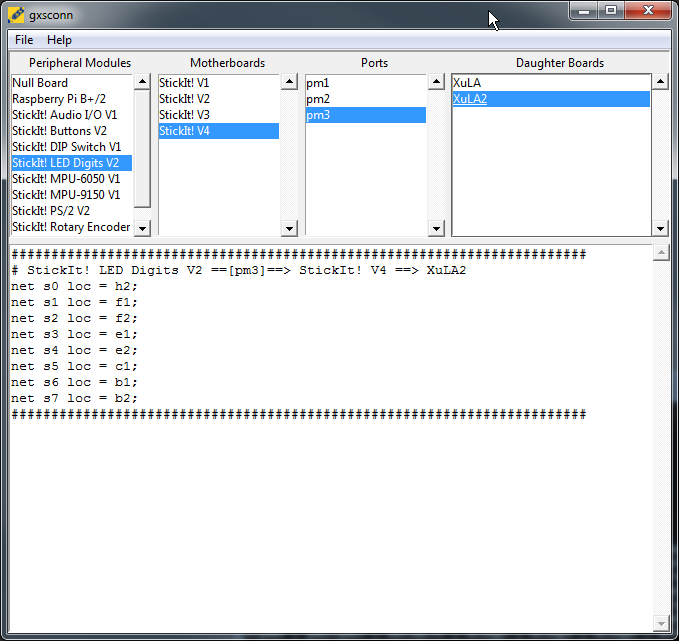
\includegraphics[width=0.7\textwidth]{gxsconn.png}}

The output from \pgm{xsconn}\ and \pgm{gxsconn}\ is formatted for use
as a UCF file in your ISE project. 


\section{Using the \rpi}

Just as with the \digpmod s, connecting the \product\ to a \rpi\ requires
you to determine the connections of the I/O signals to the pins of the FPGA.
And, once again, there's a hard way and an easy way to do that.

\subsection{The Hard Way}

Manually tracing the connections of the \rpi\ I/O signals to the pins of the FPGA
is done as follows:

\begin{itemize}
\item Use the \hyperref[tab:ChanneltoGPIOConnections]{table} on page~\pageref{tab:ChanneltoGPIOConnections} to determine 
	which \rpi\ I/O signal terminates on each channel of the \xula\ socket.
\item Find which FPGA pin of the \xula\ connects to each channel using the
	\hyperref[tab:ChanneltoFPGAConnections]{table} on page~\pageref{tab:ChanneltoFPGAConnections}.
\item Make a UCF file associating each FPGA pin with each \rpi\ I/O.
\item Include the UCF file in your Xilinx ISE FPGA project.
\end{itemize}

\subsection{The Easy Way}

Use |xsconn| or |gxsconn| just like with the \digpmod s.
Set the \rpi\ as the peripheral board and select GPIO as the port
and you'll get a complete list of the connections to the FPGA.

\subsection{Configuring the \rpi\ GPIO \label{sec:GPIOConfig}}

Most HATs perform a specific function that requires communicating with the \rpi\
through a fixed set of GPIO pins.
The \rpi\ reads the list of pins from the EEPROM on the HAT and configures
its I/O pins appropriately.

But the \xula\ and \product\ do not perform one fixed function: they can be
programmed for many types of applications.
Therefore, the list of GPIO pins used by a particular application has to be written
into the EEPROM on the \product.
This is done as follows:

\begin{enumerate}
\item Create your FPGA application for the \xula\ along with the
	required pin assignments for communicating through the GPIO connector.
\item Attach the \product\ to the GPIO connector and place a shunt on 
	the WP jumper to enable	writing to the EEPROM.
	(A \xula\ can be inserted into the J1 socket at this point, but it
	should not have a bitstream loaded into its flash memory that might
	cause the FPGA to drive the pins of the GPIO connector.)
\item Download the code from 
	\url{https://github.com/raspberrypi/hats/tree/master/eepromutils}
	onto your \rpi.
\item Edit the \filename{eeprom\_settings.txt}\ file to reflect how the GPIO
	pins are used by your application.
\item Compile the \filename{eepmake.c}\ program and then run it to create
	a binary data file that stores your GPIO pin settings:
	\begin{lstlisting}
	eepmake eeprom_settings.txt eeprom_settings.bin
	\end{lstlisting}
\item Execute the \filename{eepflash.sh}\ shell program to write the
	binary data file to the EEPROM:
	\begin{lstlisting}
	eepflash -w -f=eeprom_settings.bin -t=-24c32
	\end{lstlisting}
\item Remove the shunt from the WP jumper and reboot the \rpi.
\end{enumerate}

After the above procedure is completed, you can load the \xula\ with the
bitstream for the application.
You can change the application as long as you don't
change how it drives the GPIO pins.
(For example, don't take a GPIO pin that was previously driving the
FPGA and reverse it so that the FPGA now drives the \rpi.)
If you do change how the GPIO pins are used, you will need to update
the \product\ EEPROM again to reflect those changes before changing the
FPGA bitstream.


\section{Using Generic Circuitry}

Instead of an \rpi, you can connect generic digital circuitry to the GPIO port.
\warning{The circuitry must interface using 3.3V logic levels. The \xula\
will not tolerate 5V logic levels.}

\subsection{The Hard Way}

Use the following procedure to determine the connections of the I/O signals
from your circuitry to the pins of the FPGA:

\begin{itemize}
\item Attach the I/O signals from the generic circuitry to pins 
	1--40 of the GPIO connector. There are 26 usable I/O pins; the rest
	are mostly power and ground pins that you can use to provide
	power to the external circuitry if desired.
\item Use the \hyperref[tab:ChanneltoGPIOConnections]{table} on 
	page~\pageref{tab:ChanneltoGPIOConnections} to determine 
	which GPIO pin connects to each channel of the \xula\ socket.
\item Find which FPGA pin of the \xula\ connects to each channel using the
	\hyperref[tab:ChanneltoFPGAConnections]{table} on 
	page~\pageref{tab:ChanneltoFPGAConnections}.
\item Make a UCF file associating each FPGA pin with an I/O signal.
\item Include the UCF file in your Xilinx ISE FPGA project.
\end{itemize}

\subsection{The Easy Way}

For generic circuitry, |xsconn| or |gxsconn| can still make the pin-tracing
process a little easier.
Just set the peripheral board to be Generic and select GPIO as the port.
Then you'll get a complete list of connections between GPIO pins 1--40 and the FPGA.
You will have to manually substitute your I/O signal names for the pin numbers in 
the list to create the final UCF file for your ISE project.



\appendix


\chapter{I/O Locations}

The connections of the \xula\ I/O channels to the \digpmod\ and \rpi\
sockets of the \product\ are shown below.

\fixedpic{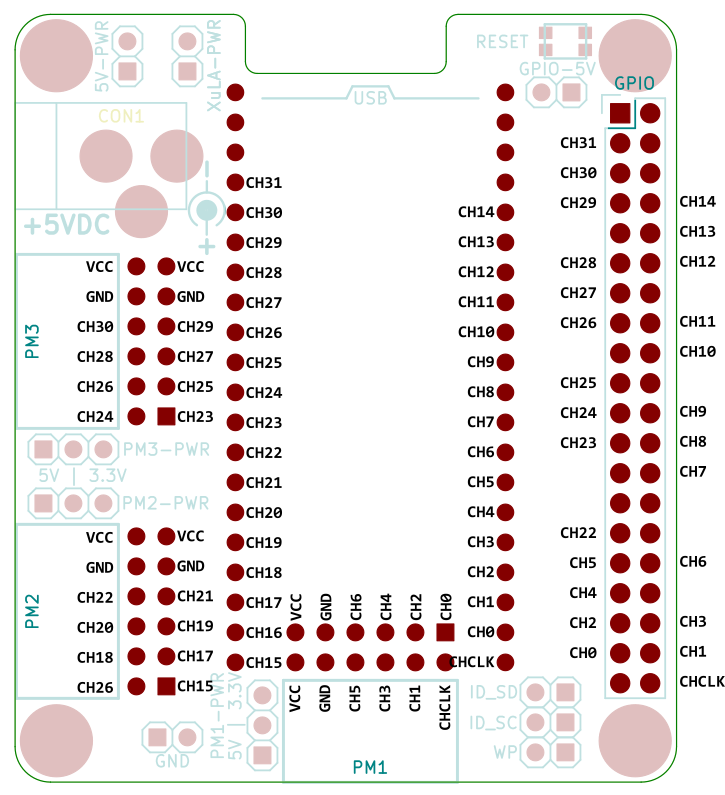
\includegraphics[width=0.7\textwidth]{channel_connects.png}}



\chapter{\ Schematic}

\pagebreak
\makebox[\textwidth][r]{\hss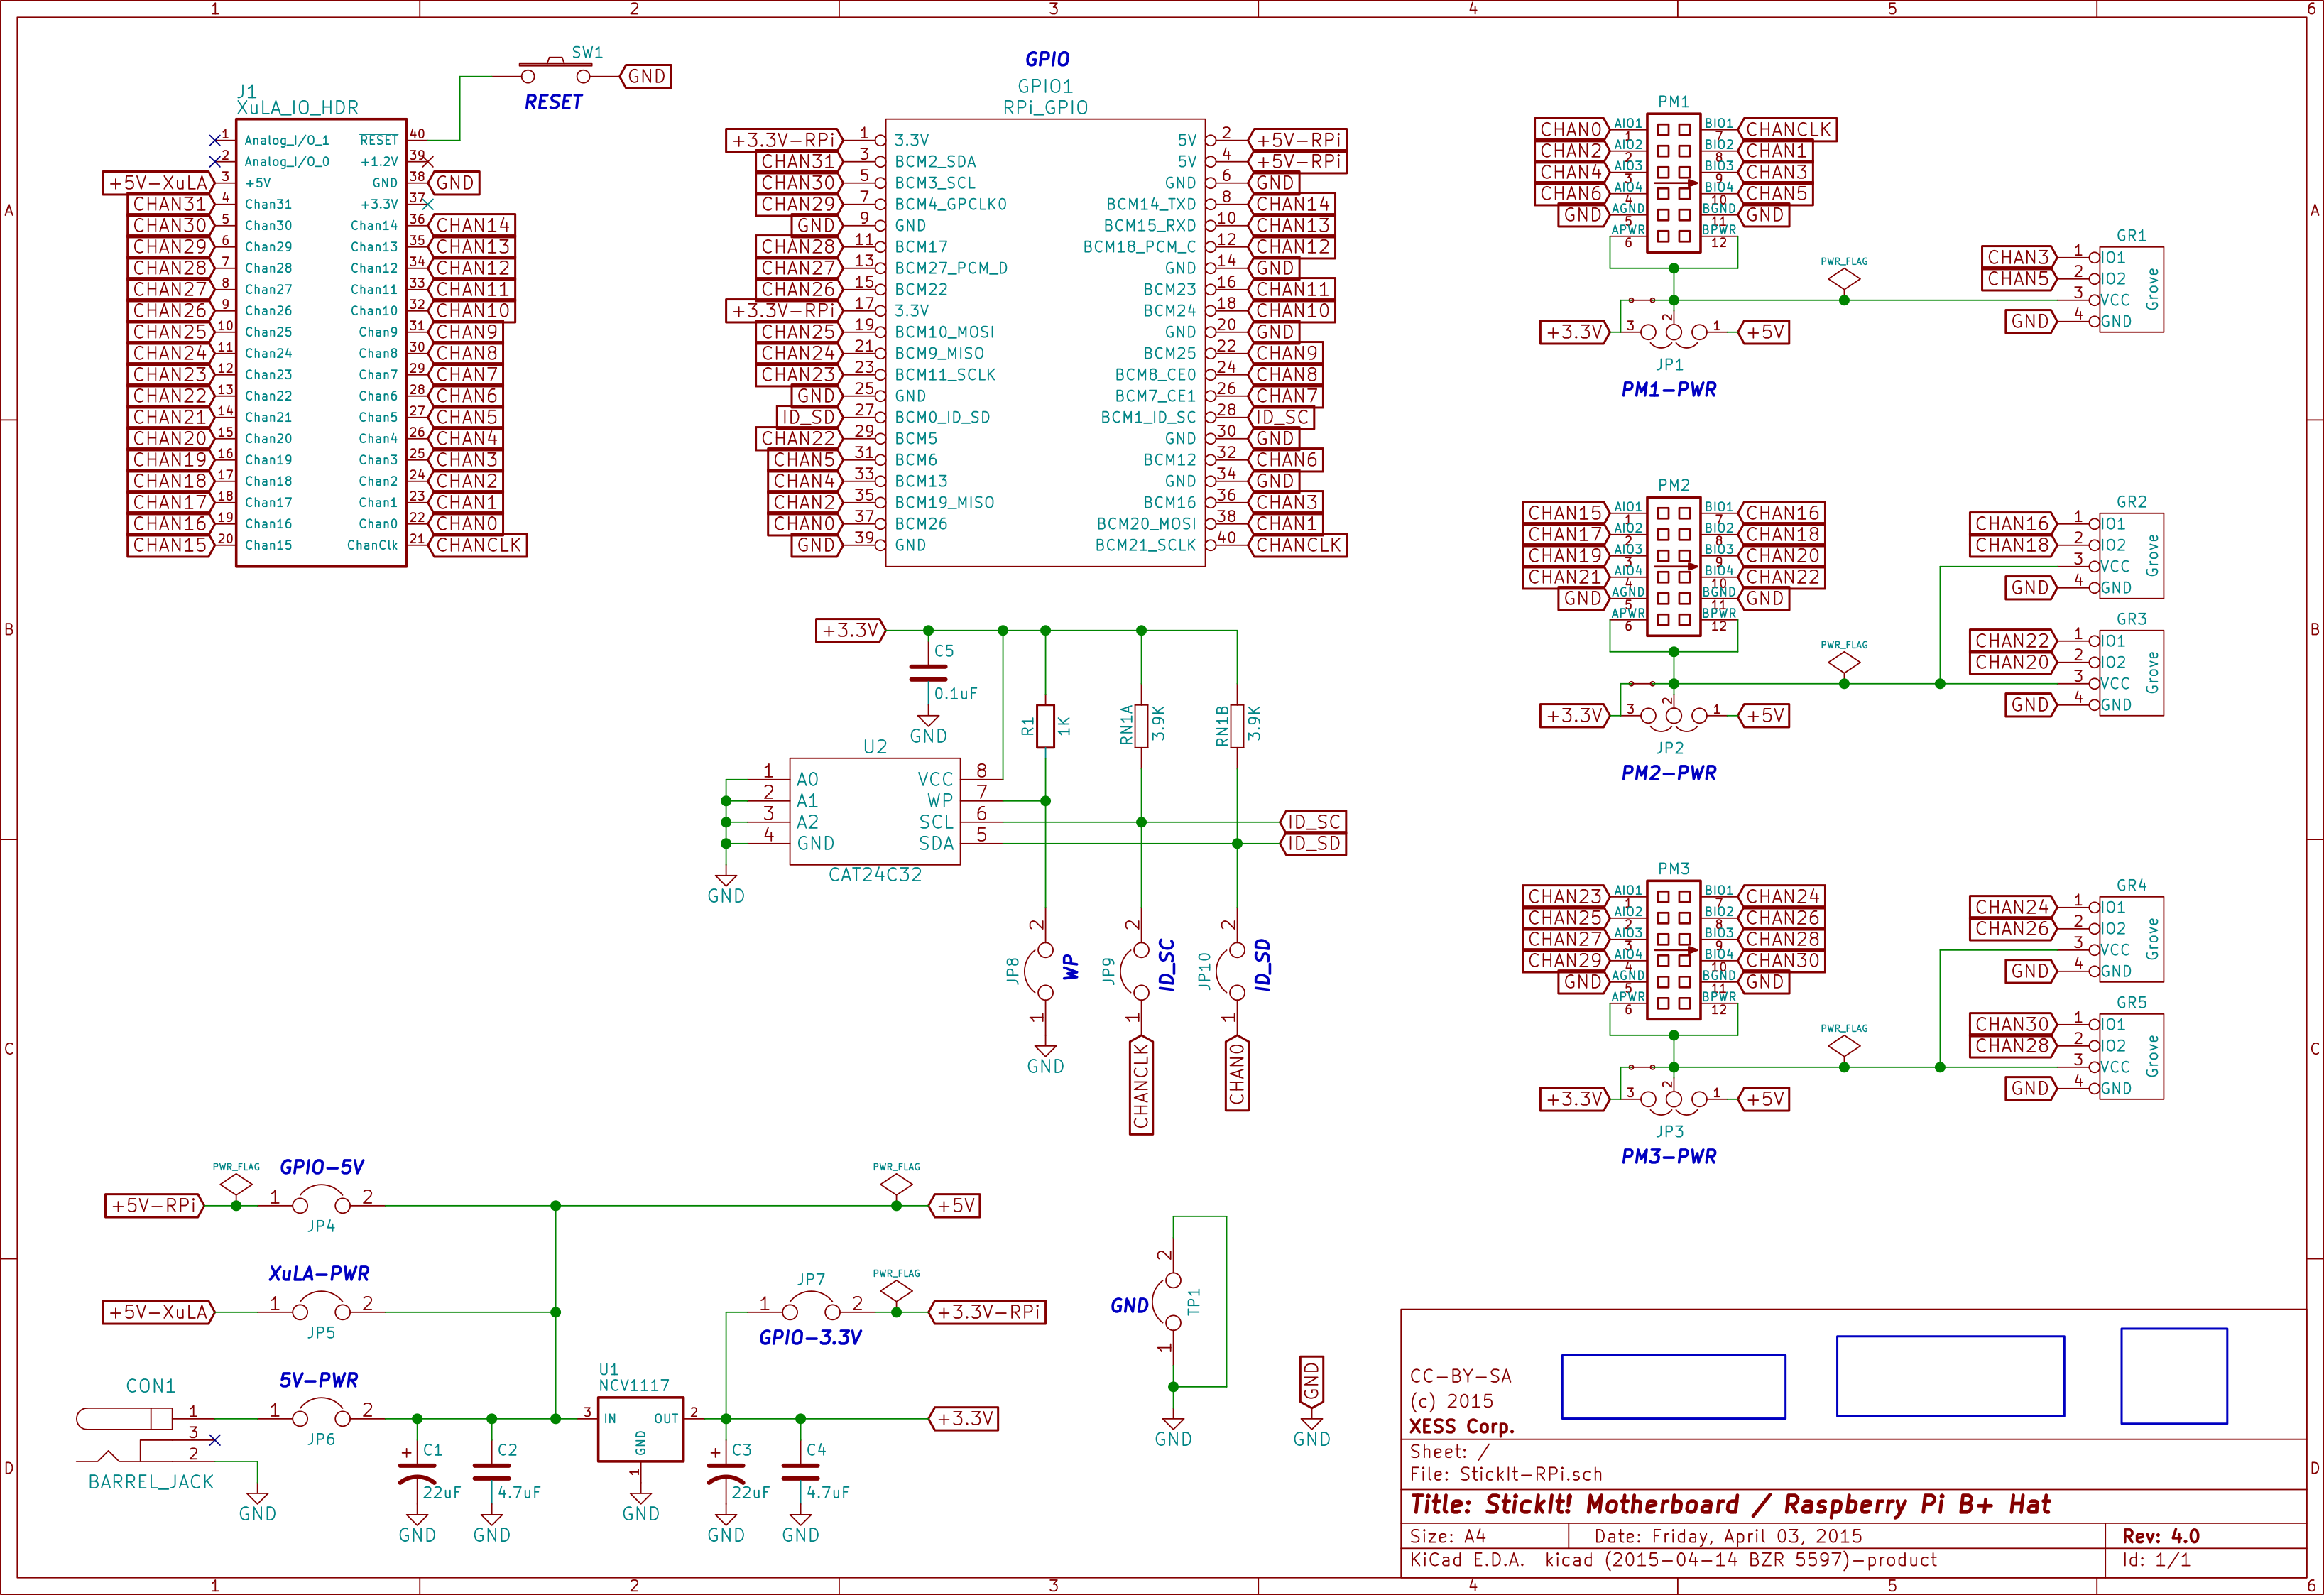
\includegraphics[width=\textheight, angle=90]{StickIt-Hat_sch.png}}
%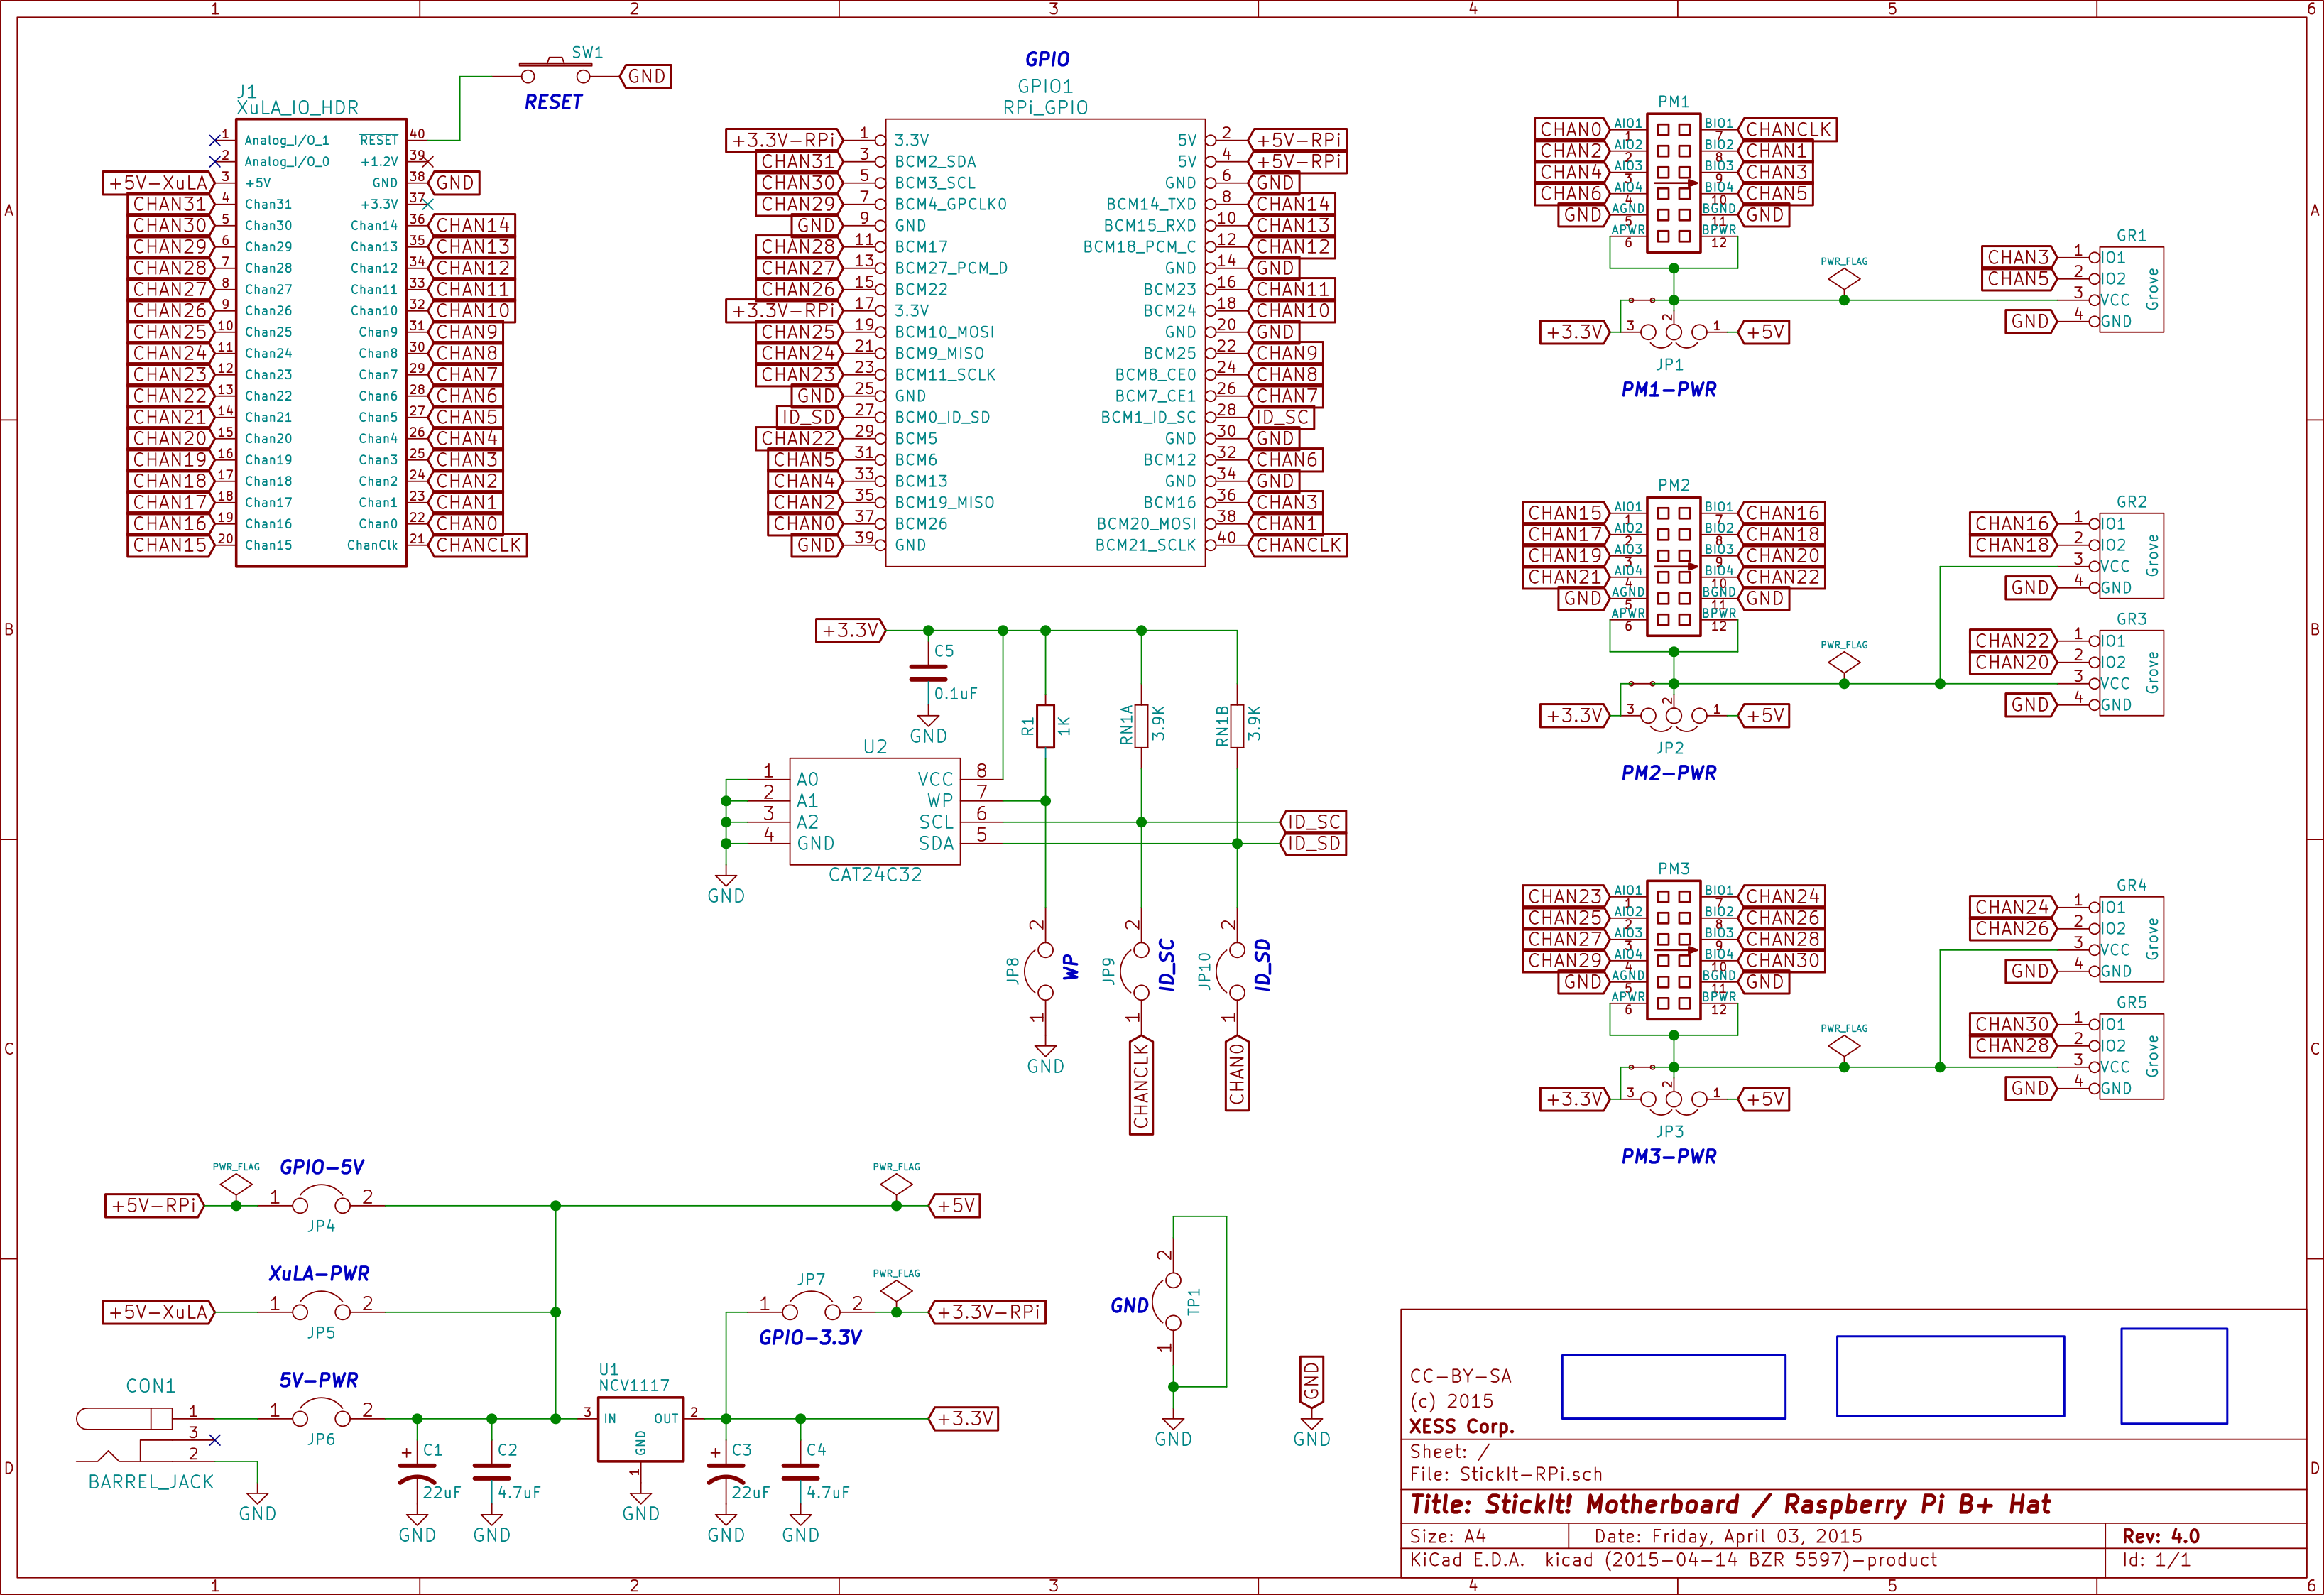
\includegraphics[width=\textheight, angle=90]{StickIt-Hat_sch.png}

\end{document}
